\begin{center}
  \textbf{3-е занятие по алгоритмам.} 
\end{center}
  Алгоритм \textbf{Эдмондса-Карпа} - это метод ФФ, но с поиском пути BFS.

  \textbf{Утв.} Расстояние(по количеству ребер) от произвольной $s$ до произвольной вершины $v$ в процессе алгоритма не уменьшается. \textbf{Доказательство.} Пусть мы ищем произвольный путь.

  \begin{center}
    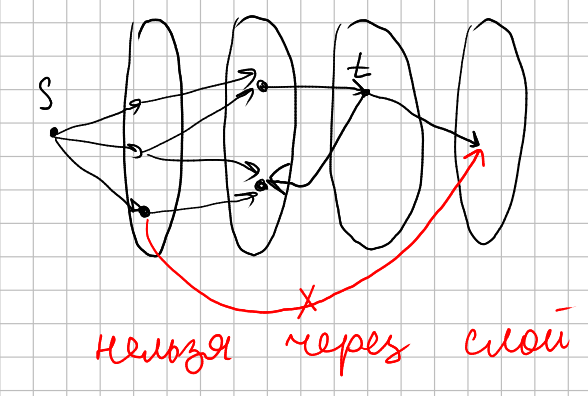
\includegraphics[scale=0.5]{img2.png}
  \end{center}
  
  Заметим, что если мы пустим поток через путь, то вершина не перескочит в слой левее, значит утверждение верно.

  Рассмотрим сколько раз могло насытиться ребро. Заметим, что если ребро насытилось несколько раз, то между этими насыщениями ребро когда-то разнасытилось, тогда рассмотрим в каких слоях находятся эти вершины.

  \begin{center}
    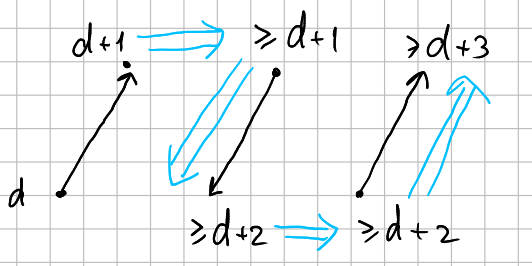
\includegraphics[scale=0.5]{img3.png}
  \end{center}

  Значит насыщений ребра могло быть только $\cfrac{V}{2}$. Ребер всего $2E$. Значит алгоритм работает за $\operatorname{O} (VE^2)$

  Давайте заметим, что если расстояние от $s$ до $t$ не увеличивается, то нам не надо перезапускать BFS.

  \textbf{Концепция блокирующих потоков} - пока у нас есть ненасыщенный путь мы находим слоистую сеть и находим блокирующий поток в слоистой сети.

  \textbf{Слоистая сеть} - это первая картинка, но мы временно игнорируем обратные ребра и внутри слоя. 

  \textbf{Блокирующий поток} - это такой поток, что мы не можем найти путь, который не содержит обратных ребер.

  Наша концепция завершится, потому что каждая итерация нашего цикла увеличивает расстояние между вершинами от $s$ до $t$, строго увеличится.

  Рассмотрим алгоритм поиска блокирующего потока. Если ребро насытилось, то мы про него забываем, если мы прошли по ребру и дальше не нашли путь до $t$, то тоже про ребро забываем. Заметим, что теперь DFS по слоистой сети работает за $V + E_{\text{удаленные}}$. Значит поиск блокирующего потока происходит за  $VE$. Чтобы забывать ребра можно как-то пронумеровать ребра исходящие из каждой вершины и еще хранить число сколько ребер мы забыли. Итоговый алгоритм работает за $O(V^2E)$

  \newpage
  \begin{center}
    \textbf{Целочисленные сети.}
  \end{center}

  \textbf{ Единичные сети.} Давайте посмотрим на алгоритм Диницы, заметим, что мы удаляем все ребра по которым прошли, значит поиск блокирующего будет за $E$. Давайте заметим, что всего итераций поиска блокирующего потока будет не больше чем $2 \sqrt{E}$. \textbf{ Доказательство } Рассмотрим сеть после $\sqrt{E}$ поиска блокирующего потока, продолжим алгоритм и посмотрим на поток, заметим что все пути больше $\sqrt{E}$, значит фаз будет не больше $\cfrac{E}{\sqrt{E}}$. Значит в итоге Диница работает за $\operatorname{O} (V \sqrt{E})$.
